\begin{figure}[t]
\centering
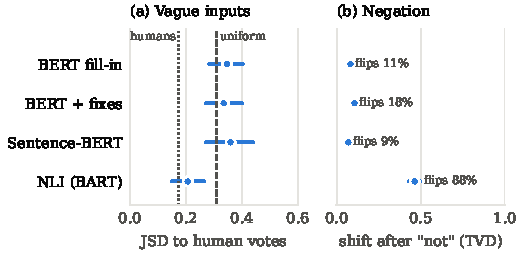
\includegraphics[width=\columnwidth]{fig1_q3.pdf}
\caption{Q3, with group descriptions. (a) Jensen--Shannon divergence between each model and the human votes (10 respondents after the attention check) on 17 vague items, with the JSD of a uniform guess and between two random halves of the respondents. (b) Total variation between a character's traits and the same traits each preceded by ``not'' (78 characters); lines are 95\% bootstrap CIs.}
\label{fig:q3}
\end{figure}
